\documentclass{beamer}

\usepackage{geometry} % Pour passer au format A4
\usepackage{graphicx} % Required for including pictures
\usepackage{float} %

\usepackage{amsmath,amsfonts,amssymb,amsthm}
\usepackage[T1]{fontenc}
\usepackage[english,francais]{babel}
\usepackage[utf8]{inputenc}
\usepackage{lmodern}
\usepackage{eurosym} % signe Euros
\usepackage{verbatim}
\usepackage{multicol}
\usefonttheme[onlymath]{serif}
\usetheme{m} 

\title{Théorème de Pythagore et sa réciproque}

\begin{document}

\frame{\titlepage}

\section{I - Un nombre au carré}
\begin{frame}
  \frametitle{I - Un nombre au carré}

  \begin{block}{1) Définition}
    Lorsqu'on multiplie un nombre par lui-même, on parle de nombre \textbf{au carré}.\\
    $8^2 = 8 \times 8 = 64$
  \end{block}

  \textbf{Vocabulaire}
  \textit{En plus de huit au carré pour $8^2$, on peut également dire :}
  \begin{itemize}	
  \item huit à la puissance 2
  \item huit exposant 2.
  \end{itemize}
  \textbf{Calculette}
  \begin{itemize}	
  \item On utilise la touche $x^2$.
  \end{itemize}
\end{frame}

\begin{frame}
  \frametitle{I - Un nombre au carré}

  \begin{exampleblock}{}
    Comment dit-on ?
  \end{exampleblock}

  \begin{itemize}	
  \item $15^2$
  \item $0.4^2$
  \item $(-5)^2$ 
  \item $AB^2$ avec AB une longueur.
  \item $O^2$
  \end{itemize}

\end{frame}

\begin{frame}
  \frametitle{I - Un nombre au carré}

  \begin{block}{}
    Remarques : Un carré est toujours positif.\\
	La multiplication de deux nombres négatifs donne un résultat positif. 
  \end{block}

  \begin{alertblock}{Attention aux calculs}
    \begin{itemize}
    \item $2^2 + 5^2 = $\\
      $7^2 = $
    \item $(3+6)^2 = $\\
      $3^2 + 6^2 = $\\
      $9^2 =$
    \item $(-4) ^2 = $\\
      $-5^2 = $
    \end{itemize}
  \end{alertblock}

\end{frame}


\begin{frame}
  \frametitle{I - Un nombre au carré}


  \begin{exampleblock}{}
    a) Quelques carrés
  \end{exampleblock}

  \begin{tabular}{| c |  c |  c |  c |    c |    c | c |}
    \hline
    -10 & -5 & -2 & -1 & -0.5 & -0.1 & 0 \\
    \hline
    \phantom{azer} & \phantom{azer} & \phantom{azer} & \phantom{azer} & \phantom{azer} & \phantom{azer} & \phantom{azer} \\       
    \hline
  \end{tabular}

  \begin{tabular}{|   c |   c | c | c | c | c | c |}
    \hline
    0.2 & 0.6 & 1 & 2 & 3 & 4 & 9 \\
    \hline
    \phantom{azer} & \phantom{azer} & \phantom{azer} & \phantom{azer} & \phantom{azer} & \phantom{azer} & \phantom{azer}\\       
    \hline
  \end{tabular}
  
  \begin{multicols}{2}
    \begin{itemize}	
    \item $(-10)^2 = $
    \item $( -5)^2 = $
    \item $( -2)^2 = $
    \item $( -1)^2 = $
    \item $( -0.5)^2 = $
    \item $( -0.1)^2 = $
    \item $ 0^2 = $
    \end{itemize}

    \begin{itemize}	
    \item $0.2^2 = $
    \item $0.6^2 = $
    \item $1^2 = $
    \item $2^2 = $
    \item $3^2 = $
    \item $4^2 = $
    \item $9^2 = $
    \end{itemize}
    
  \end{multicols}
\end{frame}


\begin{frame}
  \frametitle{I - Un nombre au carré}

  \begin{block}{}
	Rappel sur le carré en géométrie.
  \end{block}


\begin{multicols}{2}

 \textbf{Définition} : Un carré est un quadrilatère dont les côtés sont de mêmes longueurs et avec 4 angles droits.\\
\textbf{Aire} : $x^2$\\
\textbf{Périmètre} : $4x$

	\begin{figure}[H]
	  \centering
	  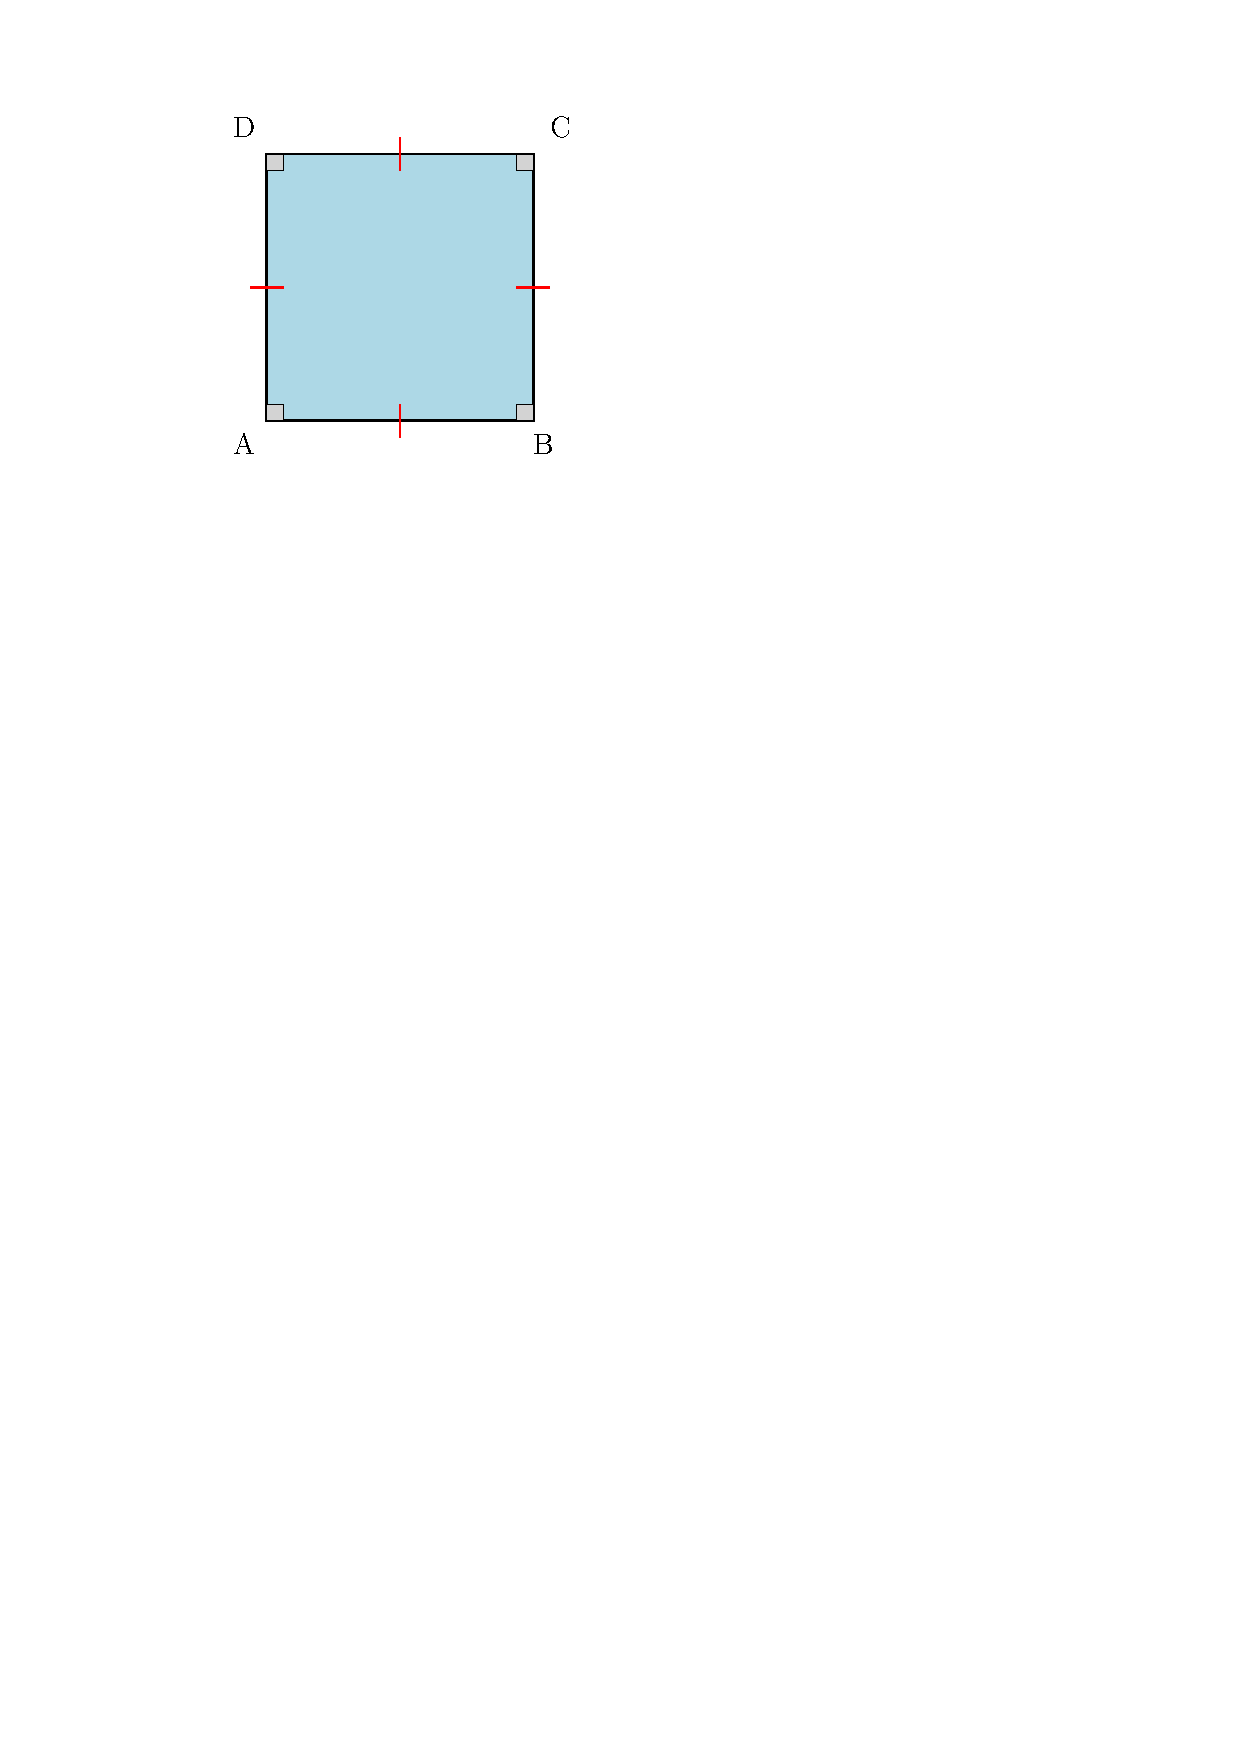
\includegraphics[width=\linewidth]{sources/1/carre.pdf}
	\end{figure}

\end{multicols}


\end{frame}


\section{II - Histoire des mathématiques}

\begin{frame}
  \frametitle{II - Histoire des mathématiques}

  \begin{block}{Pythagore de Samos}
    \vspace{4cm}
  \end{block}
\end{frame}


\section{III - Caractérisation du triangle rectangle}

\begin{frame}
  \frametitle{III - Caractérisation du triangle rectangle}

  \begin{block}{1) Propriété de Pythagore}
    Dans un triangle \textbf{rectangle}, le carré de l’hypoténuse est égal à la somme des carrés des autres 
côtés.
  \end{block}

  \begin{alertblock}{2) Énoncé exercice}
	\begin{multicols}{2}
    Soit un triangle ABC rectangle en B. 
	$$AB^2 + BC^2 = AC^2$$

	\begin{figure}[H]
	  \centering
	  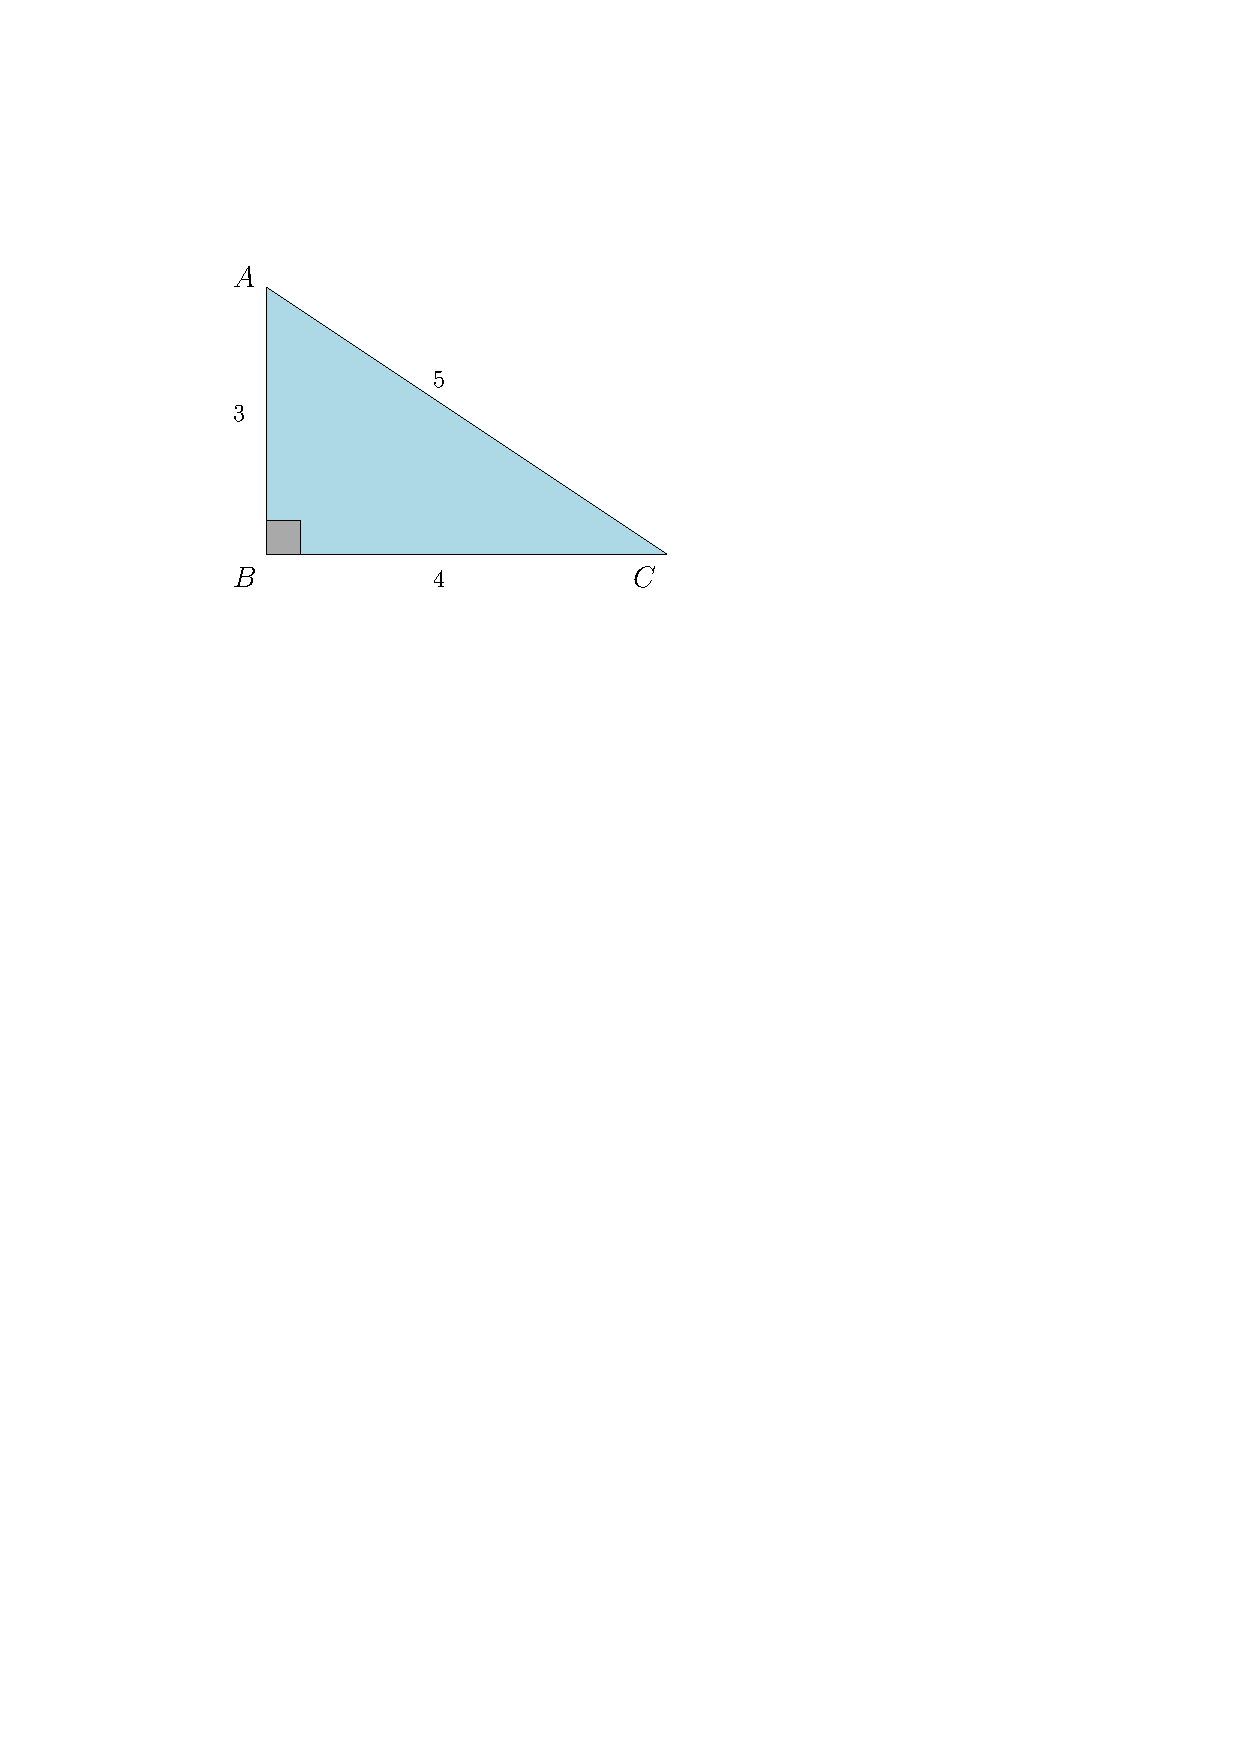
\includegraphics[width=\linewidth]{sources/1/tri-pytha.pdf}
	\end{figure}

	\end{multicols}
  \end{alertblock}
\end{frame}

\begin{frame}
  \frametitle{III - Caractérisation du triangle rectangle}

  \begin{block}{}
	Démonstration géométrique
  \end{block}

	\begin{multicols}{2}
    	\begin{figure}[H]
	  \centering
	  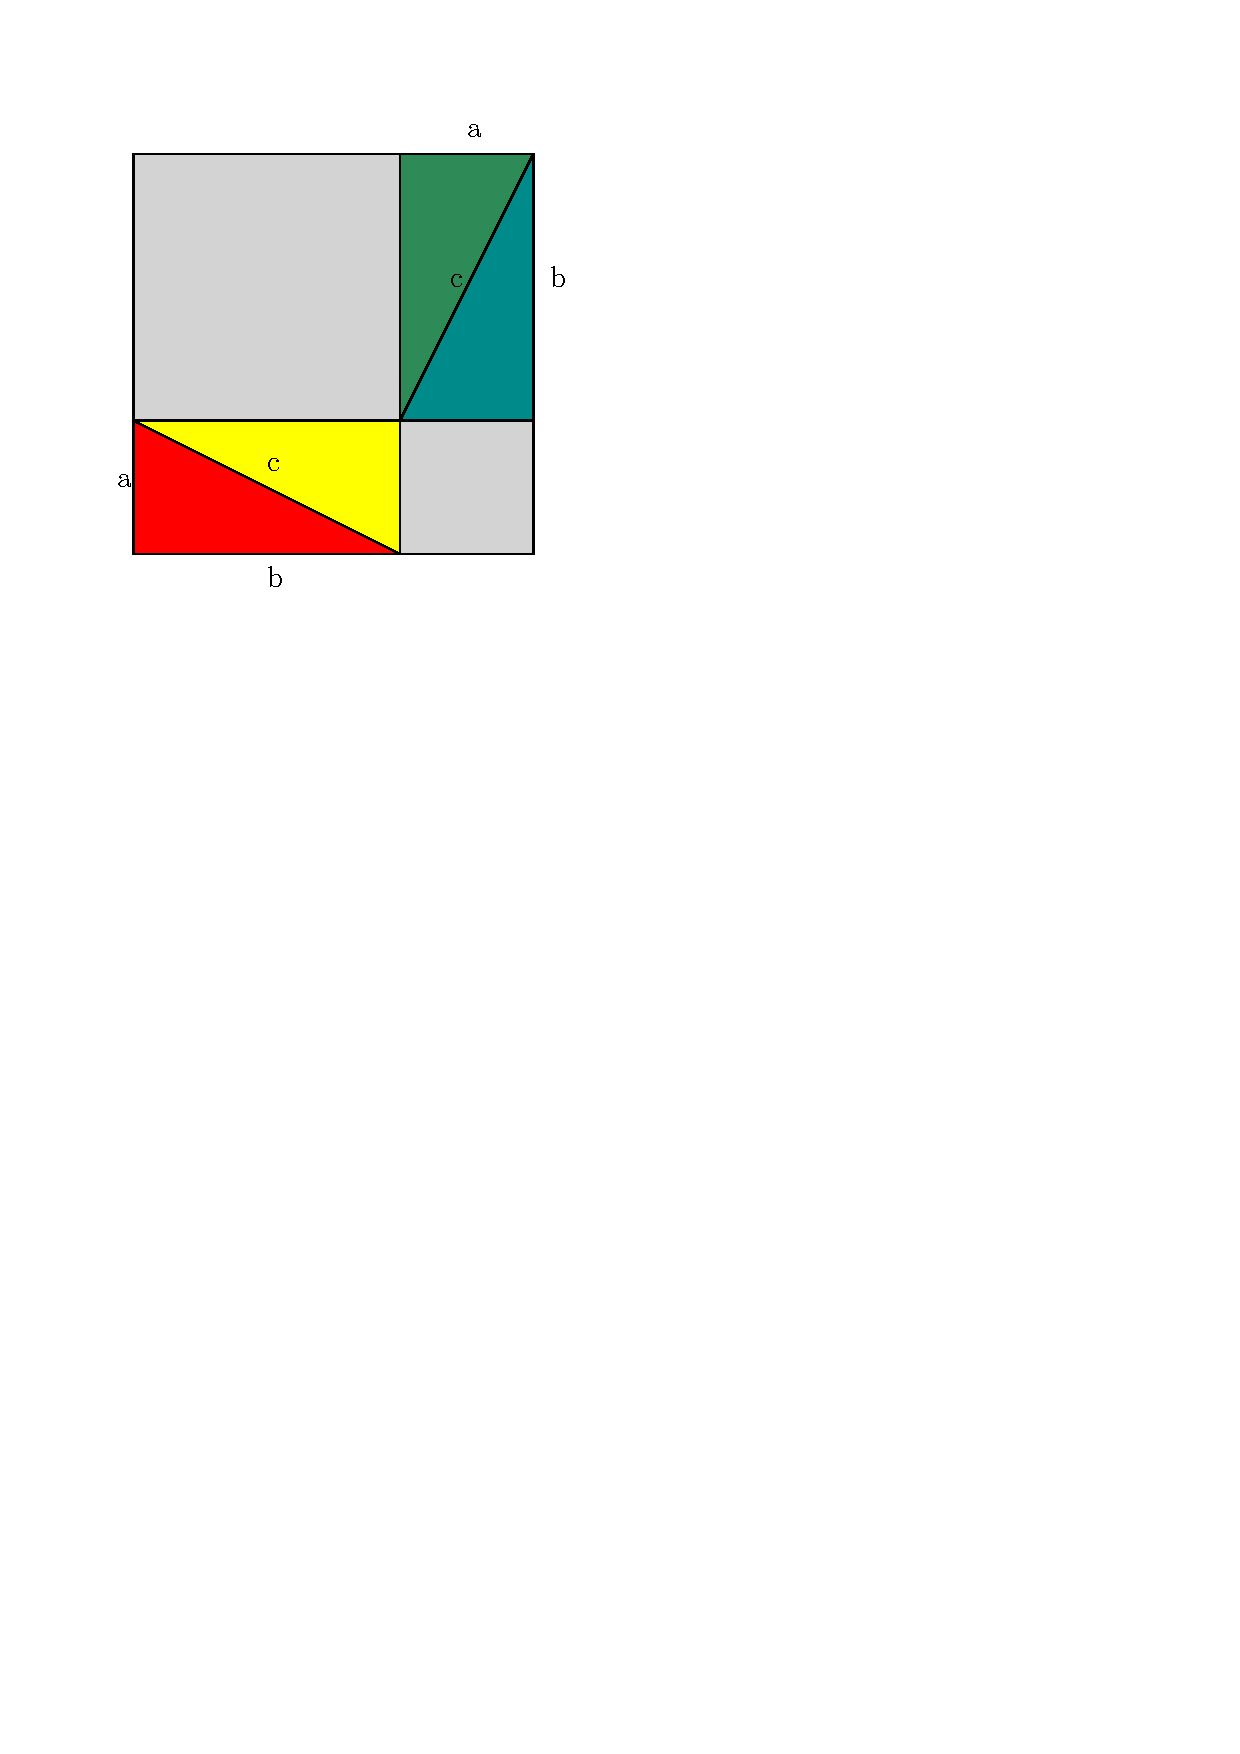
\includegraphics[width=\linewidth]{sources/1/demo-pytha-1.pdf}
	\end{figure}
    	\begin{figure}[H]
	  \centering
	  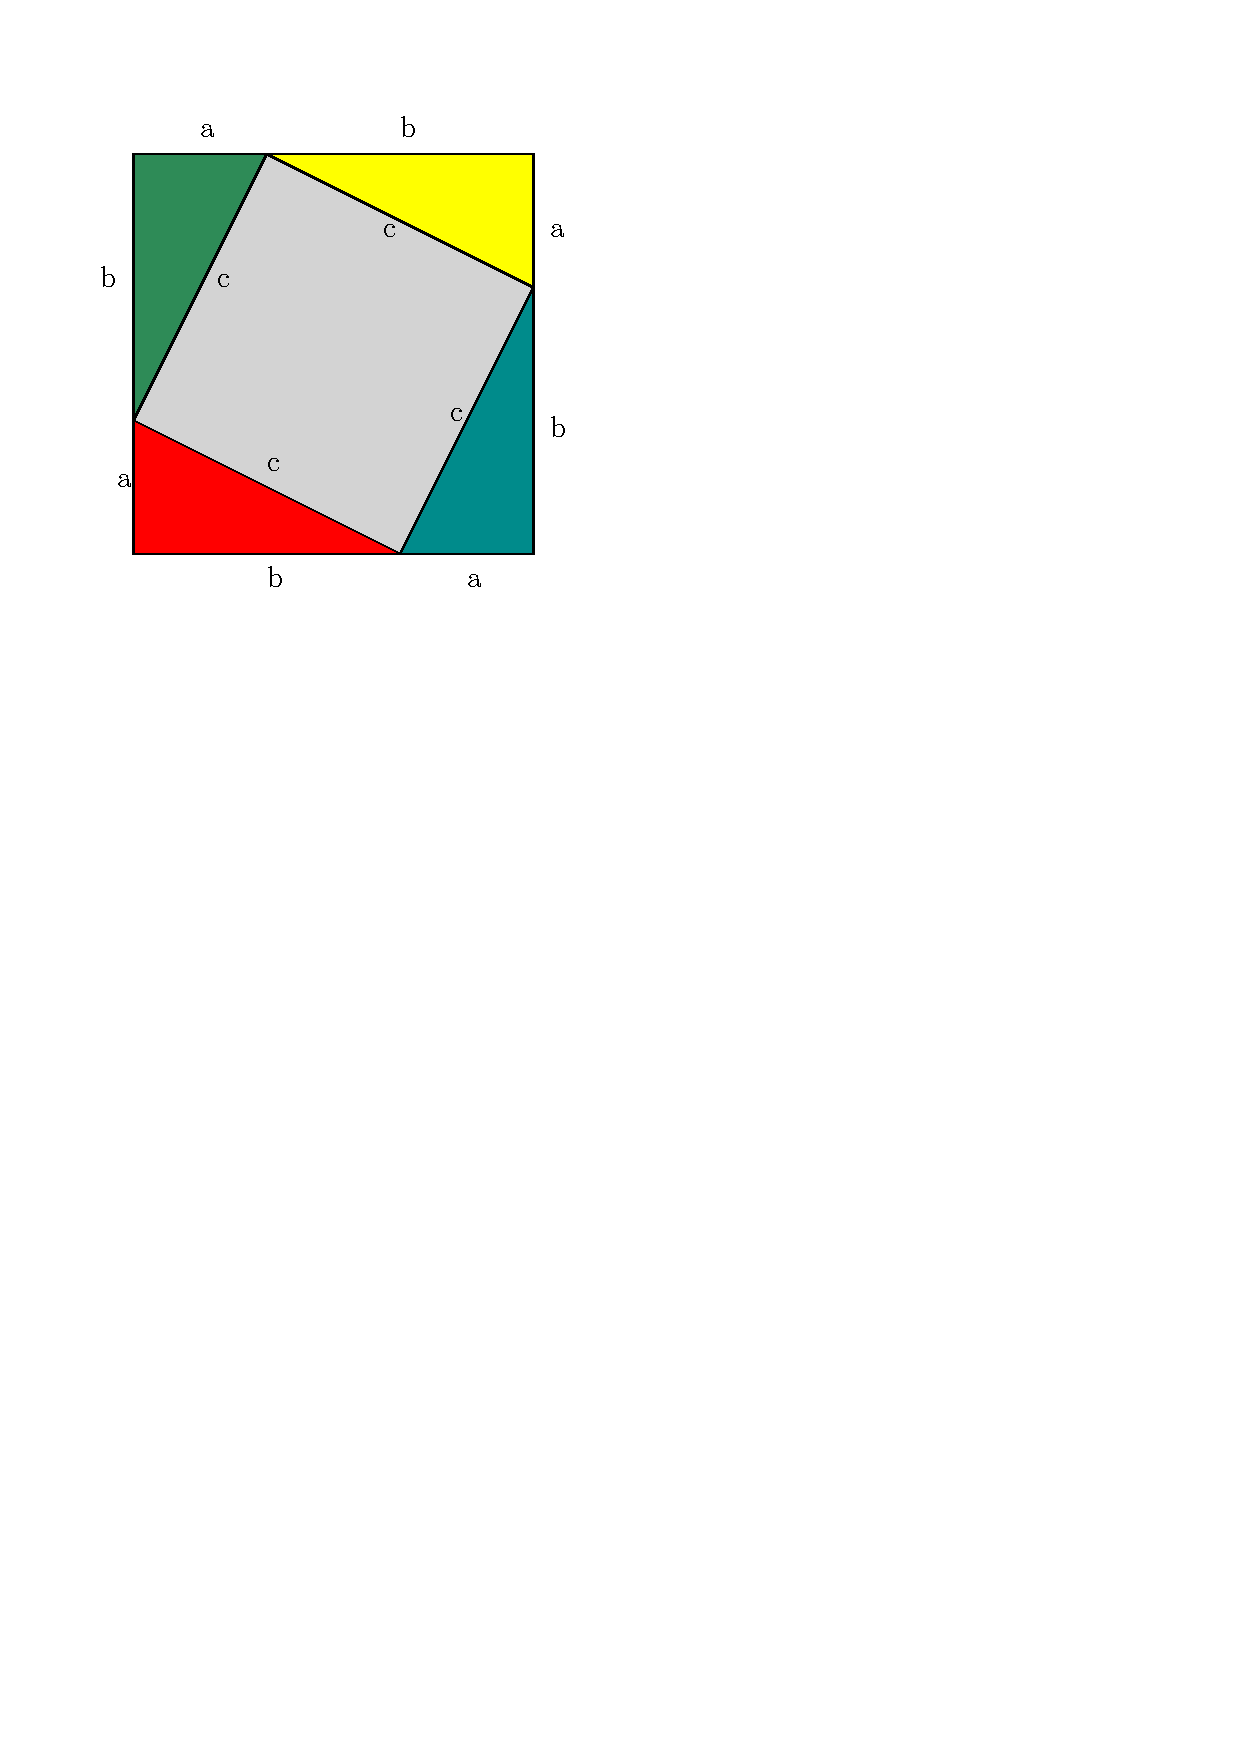
\includegraphics[width=\linewidth]{sources/1/demo-pytha-2.pdf}
	\end{figure}
	\end{multicols}


\end{frame}

\begin{frame}
  \frametitle{III - Caractérisation du triangle rectangle}

  \begin{block}{3) Utilisations}
        \begin{itemize}	
    \item Prouver qu'un triangle est rectangle
    \item Prouver qu'un triangle n'est pas rectangle. 
    \item Calculer la troisième longueur d'un triangle rectangle à l'aide de la racine carré. (Réciproque)
    \end{itemize}
  \end{block}


\end{frame}

\section{IV - Racine carré d'un nombre}

\begin{frame}
  \frametitle{IV - Racine carré d'un nombre}

  \begin{block}{1) Définition}
    Le nombre qui mis au carré donne 121 s’appelle \textbf{la racine carrée} de 121. On le note $\sqrt{121}$ = 11.
  \end{block}

  \textbf{Vocabulaire}
  \textit{On dit racine de 121.}

  \textbf{Calculette}
  \begin{itemize}	
  \item On utilise la touche $\sqrt{x}$.
  \end{itemize}
\end{frame}


\begin{frame}
  \frametitle{IV - Racine carré d'un nombre}

  \begin{block}{}
    Remarques : 
    \begin{itemize}
    	\item Les nombres dont on cherche la racine sont toujours \textbf{positifs}.
	\item certaines racines ne peuvent être écrites sous forme de fraction.
    	\item La recherche de racine est loin d'être facile et fait partie de l'histoire antique et moderne des mathématiques.
    \end{itemize} 
  \end{block}

  \begin{alertblock}{Attention aux calculs}
    \begin{itemize}
    \item $\sqrt{2 + 5} = $\\
      $\sqrt{2} + \sqrt{5}= $

    \item $\sqrt{-4} = $\\

    \end{itemize}
  \end{alertblock}
\end{frame}


\begin{frame}
  \frametitle{IV - Racine carré d'un nombre}


  \begin{exampleblock}{}
    a) Quelques racines carrés
  \end{exampleblock}

  \begin{tabular}{| c |   c | c | c | c | c |    c | c |}
    \hline
    0 & 0.2 & 1 & 2 & 4 & 9 & 30.2 & 104 \\
    \hline
    \phantom{azer} & \phantom{azer} & \phantom{azer} & \phantom{azer} & \phantom{azer} & \phantom{azer} & \phantom{azer} & \phantom{azer}\\       
    \hline
  \end{tabular}
  \begin{multicols}{2}
    \begin{itemize}	
    \item $ \sqrt{0} =$
    \item $ \sqrt{0.2} =$
    \item $ \sqrt{1} =$
    \item $ \sqrt{2} =$
    \item $ \sqrt{4} =$
    \item $ \sqrt{9} =$
    \item $ \sqrt{30.2} =$
    \item $ \sqrt{104} =$
    \end{itemize}
  \end{multicols}

\end{frame}


\end{document}
